\documentclass[conference,a4paper]{IEEEtran}

\usepackage[T1]{fontenc}
\usepackage[utf8]{inputenc}
\usepackage[indonesian]{babel}
\usepackage{cite}
\usepackage{amsmath,amssymb}
\usepackage{graphicx}
\usepackage{array}
\usepackage{booktabs}
\usepackage{tikz}
\usetikzlibrary{positioning,arrows.meta}

\graphicspath{{figures/}}
\providecommand{\IEEEkeywordsname}{Index Terms}

% Label berbahasa Indonesia. Diatur saat dokumen dimulai agar tidak ditimpa babel.
\AtBeginDocument{%
  \renewcommand{\abstractname}{Abstrak}%
  \renewcommand{\IEEEkeywordsname}{Kata Kunci}%
  \renewcommand{\figurename}{Gbr.}%
  \renewcommand{\tablename}{Tabel}%
  \renewcommand{\refname}{Referensi}%
}

\begin{document}

\title{Analisis Komparatif Temporal Convolutional Network dan Arsitektur Rekuren untuk Peramalan Harga Bitcoin dengan Fitur Waktu Siklis dan Evaluasi Baseline}

\author{%
\IEEEauthorblockN{Muhammad Farras, Nandana Bahaghani, Althaf Syakir,\\
Iqdam Shidqi, Putri Amalia}
\IEEEauthorblockA{\textit{Sains Data}\\
\textit{Institut Teknologi Sepuluh Nopember}}
}

\maketitle

\begin{abstract}
Penelitian ini membandingkan Recurrent Neural Network (RNN), Long Short-Term Memory (LSTM), dan Temporal Convolutional Network (TCN) untuk memprediksi harga penutupan Bitcoin satu hari ke depan. Data yang digunakan adalah harga harian BTC-USD dari 17 September 2014 hingga 4 Desember 2025, dengan total 4.097 observasi. Setiap model menerima window 60 hari yang berisi harga penutupan dan fitur waktu siklis berbasis sinus dan kosinus. Pelatihan diulang dengan lima random seed, lalu kinerja diukur dengan RMSE, MAE, dan sMAPE pada 808 target test yang tersusun kronologis. Berbeda dari perbandingan antarmodel saja, penelitian ini juga menguji semua model terhadap baseline persistence, yaitu prediksi bahwa harga besok sama dengan harga hari ini. Interpretabilitas ditelaah dengan SHAP pada TCN dan t-SNE pada lapisan laten ketiga model. TCN mencatat error rata-rata terendah, dengan RMSE 3.180,83 USD, MAE 2.450,17 USD, dan sMAPE 3,320\%. Namun, tidak satu pun dari 15 run model mengalahkan baseline persistence, yang mencatat RMSE 1.913,46 USD. Pada periode test ini, keunggulan TCN hanya berlaku terhadap RNN dan LSTM.
\end{abstract}

\begin{IEEEkeywords}
Bitcoin, peramalan deret waktu, Temporal Convolutional Network, LSTM, baseline persistence, fitur waktu siklis, SHAP, t-SNE
\end{IEEEkeywords}

\section{Pendahuluan}

\subsection{Latar Belakang}
Bitcoin, yang diperkenalkan oleh Nakamoto~\cite{nakamoto2008}, merupakan aset digital dengan pergerakan harga yang sangat volatil. Volatilitas ini membuat peramalan harga menarik sekaligus sulit, baik bagi peneliti maupun pelaku pasar.

Deep learning banyak digunakan untuk peramalan deret waktu karena mampu mempelajari pola non-linier dari data~\cite{lim2021}. RNN dan LSTM memproses data secara berurutan, sedangkan TCN memakai konvolusi kausal berdilatasi yang dapat dihitung secara paralel~\cite{bai2018}. Perbedaan ini mendorong pertanyaan tentang arsitektur mana yang lebih sesuai untuk harga Bitcoin.

Namun, peringkat antarmodel belum menjawab apakah sebuah model benar-benar berguna. Harga harian aset cenderung dekat dengan harga hari sebelumnya, sehingga grafik prediksi dapat tampak menempel pada harga aktual walaupun model hanya mengikuti harga terakhir. Karena itu, penelitian ini menambahkan baseline persistence sebagai pembanding dasar~\cite{hyndman2021}.

\subsection{Rumusan Masalah}
\begin{enumerate}
\item Bagaimana perbandingan kinerja RNN, LSTM, dan TCN berdasarkan RMSE, MAE, dan sMAPE?
\item Apakah ketiga model menghasilkan error yang lebih rendah daripada baseline persistence?
\item Seberapa stabil kinerja setiap model pada lima random seed?
\item Fitur apa yang paling memengaruhi prediksi TCN menurut SHAP?
\item Apakah representasi laten setiap model memisahkan hari dengan harga naik dan harga turun?
\end{enumerate}

\subsection{Tujuan Penelitian}
\begin{enumerate}
\item Membangun dan mengevaluasi RNN, LSTM, dan TCN pada data harian BTC-USD.
\item Mengukur nilai tambah setiap model terhadap baseline persistence.
\item Menelaah perilaku model melalui SHAP, t-SNE, dan aktivasi lapisan konvolusi.
\end{enumerate}

\subsection{Kontribusi}
\begin{enumerate}
\item Perbandingan tiga arsitektur dengan pengaturan pelatihan yang sama dan lima random seed.
\item Evaluasi terhadap baseline persistence pada target test yang sama.
\item Pemisahan yang jelas antara temuan yang didukung pengukuran dan yang masih bersifat indikatif.
\end{enumerate}

\subsection{Batasan}
Penelitian ini memprediksi harga satu hari ke depan dan tidak menguji strategi perdagangan. Fitur waktu siklis digunakan pada semua model, tanpa eksperimen pembanding. Oleh karena itu, kontribusi fitur tersebut terhadap akurasi tidak dapat disimpulkan secara kausal.

\section{Tinjauan Pustaka}

\subsection{Recurrent Neural Network}
RNN memproses urutan langkah demi langkah dan menyimpan ringkasan masa lalu dalam hidden state~\cite{elman1990}. Pada urutan panjang, RNN standar rentan terhadap vanishing gradient~\cite{bengio1994}.
\begin{equation}
h_t = \tanh(W_h h_{t-1} + W_x x_t + b)
\label{eq:rnn}
\end{equation}

\subsection{Long Short-Term Memory}
LSTM menambahkan sel memori yang diatur oleh input gate dan output gate~\cite{hochreiter1997}, lalu dilengkapi forget gate pada pengembangan berikutnya~\cite{gers2000}. Mekanisme ini membantu model mempertahankan informasi lebih lama daripada RNN standar.
\begin{equation}
C_t = f_t \odot C_{t-1} + i_t \odot \tilde{C}_t
\label{eq:lstm}
\end{equation}
Pada \eqref{eq:lstm}, $C_t$ adalah sel memori, $f_t$ adalah forget gate, dan $i_t$ adalah input gate.

\subsection{Temporal Convolutional Network}
TCN menyusun konvolusi kausal berdilatasi sehingga prediksi hanya bergantung pada masa lalu~\cite{bai2018}. Faktor dilatasi $d$ memperluas jangkauan historis tanpa menambah jumlah parameter secara drastis. Koneksi residual membantu aliran gradien pada jaringan yang lebih dalam.
\begin{equation}
F(s) = \sum_{i=0}^{k-1} f(i) \cdot x_{s-d \cdot i}
\label{eq:tcn}
\end{equation}

\subsection{Fitur Waktu Siklis}
Nilai waktu seperti bulan bersifat melingkar, sehingga bulan 12 sebenarnya dekat dengan bulan 1. Transformasi sinus dan kosinus mempertahankan kedekatan tersebut, dengan $t$ sebagai nilai waktu dan $P$ sebagai panjang siklus.
\begin{equation}
x_{\sin} = \sin\left(\frac{2\pi t}{P}\right), \quad x_{\cos} = \cos\left(\frac{2\pi t}{P}\right)
\label{eq:siklis}
\end{equation}

\subsection{Baseline Persistence}
Baseline persistence, atau naive forecast, memakai nilai terakhir sebagai prediksi berikutnya~\cite{hyndman2021}. Metode ini tidak memerlukan pelatihan. Metode ini tidak berkaitan dengan algoritma Naive Bayes.
\begin{equation}
\hat{y}_t = y_{t-1}
\label{eq:baseline}
\end{equation}
Pembanding ini relevan karena hipotesis pasar efisien menyatakan bahwa harga aset sudah mencerminkan informasi yang tersedia~\cite{fama1970}. Jika hipotesis tersebut berlaku, perubahan harga harian sulit diprediksi dari harga masa lalu.

\subsection{Metrik Evaluasi}
RMSE memberi penalti lebih besar pada error besar, sedangkan MAE lebih mudah ditafsirkan sebagai rata-rata error dalam USD~\cite{hodson2022}. sMAPE menyatakan error secara relatif terhadap besarnya nilai aktual dan prediksi~\cite{hyndman2006}.
\begin{equation}
\mathrm{RMSE} = \sqrt{\frac{1}{n}\sum_{t=1}^{n}\left(y_t - \hat{y}_t\right)^2}
\label{eq:rmse}
\end{equation}
\begin{equation}
\mathrm{MAE} = \frac{1}{n}\sum_{t=1}^{n}\left|y_t - \hat{y}_t\right|
\label{eq:mae}
\end{equation}
\begin{equation}
\mathrm{sMAPE} = \frac{100\%}{n}\sum_{t=1}^{n}\frac{2\left|y_t - \hat{y}_t\right|}{\left|y_t\right| + \left|\hat{y}_t\right|}
\label{eq:smape}
\end{equation}

\subsection{Interpretabilitas}
SHAP membagi kontribusi prediksi kepada setiap fitur berdasarkan nilai Shapley~\cite{lundberg2017}. t-SNE memetakan data berdimensi tinggi ke dua dimensi dengan menjaga kedekatan lokal~\cite{vandermaaten2008}. Jarak antarkelompok pada peta t-SNE tidak selalu bermakna, sehingga hasilnya perlu dibaca secara hati-hati.

\section{Metodologi}
Penelitian mengikuti satu alur yang sama untuk ketiga model, dan baseline dihitung pada target test yang identik, seperti ditunjukkan pada Gbr.~\ref{fig:alur}. Model memakai data train dan test, sedangkan baseline hanya memakai harga terakhir pada setiap window test.

\begin{figure}[!t]
\centering
\begin{tikzpicture}[
  node distance=3mm and 4mm,
  kotak/.style={draw, thin, align=center, font=\footnotesize, inner sep=2.5pt, minimum height=8mm},
  penuh/.style={kotak, text width=75mm},
  separuh/.style={kotak, text width=35.5mm},
  panah/.style={-{Latex[length=1.5mm]}, thin}
]
\node[penuh] (data) {\textbf{Data BTC-USD harian}\\4.097 observasi};
\node[penuh, below=of data] (fitur) {\textbf{Fitur waktu siklis}\\sinus dan kosinus untuk tahun dan bulan};
\node[penuh, below=of fitur] (norm) {\textbf{Normalisasi}\\MinMaxScaler, fit pada 80\% data awal};
\node[penuh, below=of norm] (window) {\textbf{Sliding window dan pembagian data}\\window 60 hari; 3.228 train dan 808 test};
\node[separuh, below=of window.south west, anchor=north west] (model) {\textbf{RNN, LSTM, TCN}\\5 seed, 30 epoch, batch 32};
\node[separuh, below=of window.south east, anchor=north east] (baseline) {\textbf{Baseline persistence}\\tanpa pelatihan};
\node[penuh, below=of model.south west, anchor=north west] (evaluasi) {\textbf{Evaluasi pada 808 target test}\\RMSE, MAE, dan sMAPE dalam USD};
\node[penuh, below=of evaluasi] (interpretasi) {\textbf{Analisis interpretabilitas}\\SHAP, t-SNE, dan aktivasi pada run RMSE terendah};
\draw[panah] (data) -- (fitur);
\draw[panah] (fitur) -- (norm);
\draw[panah] (norm) -- (window);
\draw[panah] (window.south -| model) -- (model);
\draw[panah] (window.south -| baseline) -- (baseline);
\draw[panah] (model) -- (evaluasi.north -| model);
\draw[panah] (baseline) -- (evaluasi.north -| baseline);
\draw[panah] (evaluasi) -- (interpretasi);
\end{tikzpicture}
\caption{Alur penelitian.}
\label{fig:alur}
\end{figure}

\subsection{Data}
Data harian BTC-USD diambil dari Yahoo Finance melalui pustaka yfinance. Tidak ada nilai kosong, tanggal ganda, atau tanggal yang terlewat pada periode penelitian. Ringkasan data ditunjukkan pada Tabel~\ref{tab:data}.

\begin{table}[!t]
\centering
\caption{Ringkasan Data}
\label{tab:data}
\footnotesize
\begin{tabular}{@{}ll@{}}
\toprule
\textbf{Aspek} & \textbf{Keterangan} \\
\midrule
Periode & 17 September 2014 -- 4 Desember 2025 \\
Frekuensi & Harian \\
Jumlah observasi & 4.097 \\
Harga penutupan terendah & 178,10 USD \\
Harga penutupan tertinggi & 124.752,53 USD \\
Target prediksi & Harga penutupan satu hari ke depan \\
\bottomrule
\end{tabular}
\end{table}

\subsection{Pra-pemrosesan}
\begin{enumerate}
\item \textbf{Fitur waktu.} Empat fitur dibuat: \texttt{year\_sin} dan \texttt{year\_cos} dengan periode 365 hari, serta \texttt{month\_sin} dan \texttt{month\_cos} dengan periode 12 bulan.
\item \textbf{Normalisasi.} MinMaxScaler ke rentang 0--1 di-fit pada 3.277 observasi pertama, atau 80\% data, lalu diterapkan ke seluruh data.
\item \textbf{Sliding window.} Setiap sampel berisi 60 hari dan 5 fitur, sehingga bentuk inputnya (60, 5).
\item \textbf{Pembagian data.} Sebanyak 4.036 sampel dibagi secara kronologis menjadi 3.228 sampel training dan 808 sampel test.
\end{enumerate}

Target test mencakup 18 September 2023 hingga 3 Desember 2025. Observasi terakhir tidak digunakan sebagai target karena batas perulangan pada fungsi pembuatan window.

\subsection{Arsitektur Model}
Ketiga model memiliki lapisan laten Dense(16) sebelum output, sehingga representasinya dapat dianalisis dengan cara yang sama. Susunan setiap model ditunjukkan pada Tabel~\ref{tab:arsitektur}.

\begin{table}[!t]
\centering
\caption{Arsitektur Model}
\label{tab:arsitektur}
\footnotesize
\begin{tabular}{@{}l>{\raggedright\arraybackslash}p{0.62\columnwidth}c@{}}
\toprule
\textbf{Model} & \textbf{Susunan lapisan} & \textbf{Parameter} \\
\midrule
RNN & SimpleRNN(64) $\rightarrow$ Dropout(0,1) $\rightarrow$ Dense(16) $\rightarrow$ Dense(1) & 5.537 \\
LSTM & LSTM(64) $\rightarrow$ Dropout(0,1) $\rightarrow$ Dense(16) $\rightarrow$ Dense(1) & 18.977 \\
TCN & Conv1D(32, kernel 1) $\rightarrow$ 6 blok residual $\rightarrow$ timestep terakhir $\rightarrow$ Dense(16) $\rightarrow$ Dense(1) & 13.217 \\
\bottomrule
\end{tabular}
\end{table}

Setiap blok residual TCN memakai konvolusi kausal dengan 32 filter, kernel 2, dan SpatialDropout 0,1. Faktor dilatasinya 1, 2, 4, 8, 16, dan 32, sehingga receptive field mencapai 64 hari dan mencakup seluruh window.

\subsection{Pelatihan}
Pengaturan pelatihan yang sama digunakan untuk semua model, seperti pada Tabel~\ref{tab:pelatihan}. Eksperimen dijalankan pada CPU dengan Python 3.10.11, TensorFlow 2.21.0, Keras 3.12.1, scikit-learn 1.7.2, dan SHAP 0.49.1.

\begin{table}[!t]
\centering
\caption{Pengaturan Pelatihan}
\label{tab:pelatihan}
\footnotesize
\begin{tabular}{@{}ll@{}}
\toprule
\textbf{Pengaturan} & \textbf{Nilai} \\
\midrule
Optimizer & Adam, learning rate 0,001 \\
Fungsi loss & Mean Squared Error \\
Epoch & 30 \\
Batch size & 32 \\
Validation split & 10\% (tanpa early stopping) \\
Random seed & 42, 123, 1234, 2023, 9999 \\
\bottomrule
\end{tabular}
\end{table}

\subsection{Evaluasi}
Prediksi dikembalikan ke skala USD sebelum RMSE, MAE, dan sMAPE dihitung. Kinerja utama dilaporkan sebagai rata-rata dan simpangan baku dari lima seed. Baseline persistence bersifat deterministik, sehingga hanya memiliki satu nilai.

Run dengan RMSE test terendah dipakai untuk plot prediksi, t-SNE, SHAP, dan aktivasi. Pemilihan ini tidak digunakan sebagai ukuran kinerja utama karena memakai data test.

\subsection{Analisis Interpretabilitas}
\begin{enumerate}
\item \textbf{SHAP.} KernelExplainer diterapkan pada TCN dengan 20 sampel background, 3 sampel test, dan nsamples 600. Nilainya dijumlahkan per fitur di seluruh timestep, lalu dikonversi ke USD.
\item \textbf{t-SNE.} Aktivasi Dense(16) pada data test direduksi menjadi dua dimensi dengan perplexity 30 dan random state 42. Titik diberi label naik (417 hari) atau turun (391 hari) berdasarkan perubahan harga target terhadap hari sebelumnya.
\item \textbf{Aktivasi.} Output lapisan konvolusi pertama TCN divisualisasikan pada sampel test terakhir.
\end{enumerate}

\section{Hasil dan Pembahasan}
TCN menjadi model terbaik di antara ketiga arsitektur, tetapi semua model masih kalah dari baseline persistence.

\subsection{Kinerja Model}
Seperti pada Tabel~\ref{tab:kinerja}, TCN mencatat error rata-rata terendah pada ketiga metrik. RMSE-nya 35,2\% lebih rendah daripada LSTM dan 56,9\% lebih rendah daripada RNN. Hasil ini sejalan dengan Bai dkk.~\cite{bai2018}, tetapi desain penelitian ini tidak mengisolasi penyebab keunggulan tersebut.

\begin{table}[!t]
\centering
\caption{Kinerja pada Data Test (Rata-rata $\pm$ Simpangan Baku dari Lima Seed)}
\label{tab:kinerja}
\footnotesize
\resizebox{\columnwidth}{!}{%
\begin{tabular}{@{}lcccc@{}}
\toprule
\textbf{Model} & \textbf{RMSE (USD)} & \textbf{MAE (USD)} & \textbf{sMAPE (\%)} & \textbf{Waktu (detik)} \\
\midrule
RNN & 7.378,45 $\pm$ 1.348,87 & 5.482,11 $\pm$ 891,13 & 6,267 $\pm$ 0,878 & 13,56 $\pm$ 0,25 \\
LSTM & 4.908,63 $\pm$ 1.212,85 & 3.920,78 $\pm$ 988,82 & 4,839 $\pm$ 0,990 & 33,34 $\pm$ 1,26 \\
TCN & 3.180,83 $\pm$ 619,28 & 2.450,17 $\pm$ 459,59 & 3,320 $\pm$ 0,579 & 23,02 $\pm$ 0,62 \\
\bottomrule
\end{tabular}%
}
\end{table}

Pelatihan TCN rata-rata berlangsung 23,02 detik, lebih cepat daripada LSTM (33,34 detik) dan lebih lambat daripada RNN (13,56 detik). Angka ini hanya berlaku untuk CPU yang digunakan, sehingga dapat berbeda pada perangkat lain.

\subsection{Stabilitas antar-Seed}
Urutan model dapat berubah menurut seed (Tabel~\ref{tab:seed}). TCN lebih baik daripada LSTM pada 4 dari 5 seed, tetapi pada seed 1234 RMSE LSTM (2.572,13 USD) lebih rendah daripada TCN (4.076,53 USD). LSTM dan TCN selalu lebih baik daripada RNN.

\begin{table}[!t]
\centering
\caption{RMSE (USD) / sMAPE (\%) Setiap Seed}
\label{tab:seed}
\footnotesize
\begin{tabular}{@{}cccc@{}}
\toprule
\textbf{Seed} & \textbf{RNN} & \textbf{LSTM} & \textbf{TCN} \\
\midrule
42 & 6.506,67 / 5,455 & 5.729,15 / 5,206 & 3.623,41 / 3,333 \\
123 & 7.989,99 / 6,711 & 5.232,18 / 5,164 & 2.334,90 / 2,599 \\
1234 & 5.685,91 / 5,263 & 2.572,13 / 3,176 & 4.076,53 / 4,312 \\
2023 & 9.618,15 / 7,676 & 5.955,93 / 6,168 & 2.731,42 / 2,919 \\
9999 & 7.091,52 / 6,229 & 5.053,77 / 4,480 & 3.137,91 / 3,436 \\
\bottomrule
\end{tabular}
\end{table}

Simpangan baku RMSE TCN adalah yang terkecil (619,28 USD). Relatif terhadap rata-ratanya, variasi RNN 18,3\%, TCN 19,5\%, dan LSTM 24,7\%. Temuan ini menunjukkan bahwa perbandingan dari satu run saja dapat menyesatkan.

\subsection{Perbandingan dengan Baseline}
Tabel~\ref{tab:baseline} menunjukkan bahwa tidak satu pun dari 15 run model mengalahkan baseline. Baseline mencatat RMSE 1.913,46 USD, MAE 1.347,06 USD, dan sMAPE 1,785\%. Run terbaik TCN pun masih memiliki RMSE 22,0\% lebih tinggi.

\begin{table}[!t]
\centering
\caption{Perbandingan Model dengan Baseline Persistence}
\label{tab:baseline}
\footnotesize
\begin{tabular}{@{}l>{\centering\arraybackslash}p{0.18\columnwidth}>{\centering\arraybackslash}p{0.18\columnwidth}>{\centering\arraybackslash}p{0.2\columnwidth}@{}}
\toprule
\textbf{Model} & \textbf{RMSE rata-rata (USD)} & \textbf{RMSE run terbaik (USD)} & \textbf{Selisih terhadap baseline (\%)} \\
\midrule
Baseline persistence & 1.913,46 & -- & -- \\
TCN & 3.180,83 & 2.334,90 & +66,2 \\
LSTM & 4.908,63 & 2.572,13 & +156,5 \\
RNN & 7.378,45 & 5.685,91 & +285,6 \\
\bottomrule
\end{tabular}
\end{table}

Pada periode test ini, model belum memberi nilai tambah dibanding memakai harga hari sebelumnya. Temuan ini tidak membuktikan bahwa harga Bitcoin sama sekali tidak dapat diprediksi, karena hanya berlaku untuk konfigurasi dan periode yang diuji. Target berupa harga mentah mungkin ikut berperan, tetapi faktor ini belum diuji secara terpisah.

\subsection{Visualisasi Prediksi}
RNN berada di bawah harga aktual pada sebagian besar periode harga tinggi, sedangkan LSTM dan TCN mengikuti harga lebih dekat (Gbr.~\ref{fig:prediksi}). Kedekatan visual ini tidak cukup untuk menilai kegunaan model. Tabel~\ref{tab:baseline} menunjukkan bahwa baseline tanpa pelatihan tetap menghasilkan error lebih rendah.

\begin{figure}[!t]
\centering
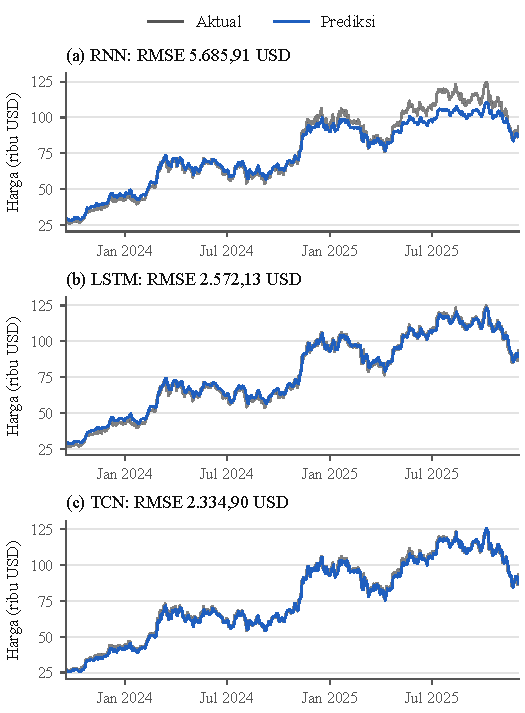
\includegraphics[width=\columnwidth]{fig2_prediksi.pdf}
\caption{Harga aktual dan prediksi pada data test, memakai run terbaik setiap model: (a) RNN, (b) LSTM, dan (c) TCN.}
\label{fig:prediksi}
\end{figure}

\subsection{Analisis SHAP}
Harga penutupan mendominasi prediksi TCN, dengan rata-rata kontribusi sekitar 55.000 USD (Gbr.~\ref{fig:shap}). Kontribusi setiap fitur waktu kurang dari sekitar 1.000 USD. Hasil ini indikatif karena hanya memakai 3 sampel, dan tidak membuktikan bahwa fitur waktu tidak berguna bagi akurasi.

\begin{figure}[!t]
\centering
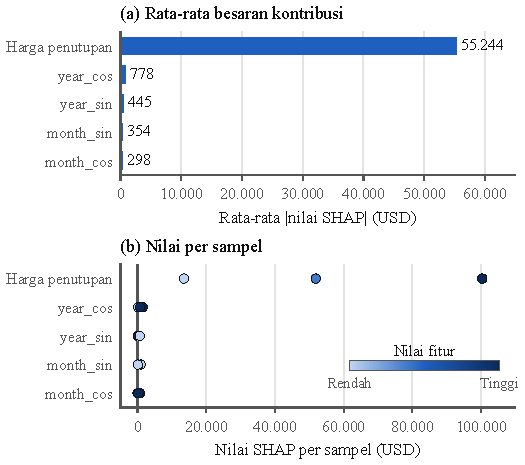
\includegraphics[width=\columnwidth]{fig3_shap.pdf}
\caption{Kontribusi fitur pada TCN dalam USD: (a) rata-rata besaran dan (b) nilai per sampel.}
\label{fig:shap}
\end{figure}

\subsection{Representasi Laten}
Ketiga model membentuk kelompok dan lintasan, tetapi titik naik dan turun tetap bercampur di dalamnya (Gbr.~\ref{fig:tsne}). Secara visual, tidak ada model yang memisahkan kedua label tersebut. Hal ini wajar karena model dilatih untuk memprediksi level harga, bukan arah perubahan. Pembacaan ini bersifat kualitatif, sehingga tidak dapat dijadikan bukti bahwa representasi satu model lebih baik.

\begin{figure}[!t]
\centering
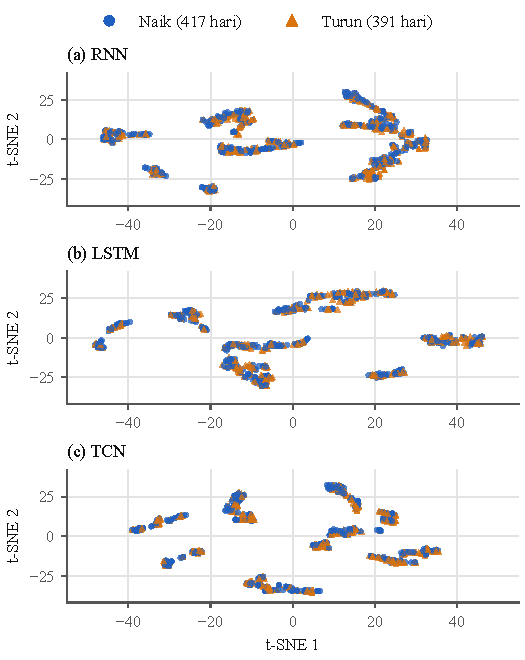
\includegraphics[width=\columnwidth]{fig4_tsne.pdf}
\caption{Peta t-SNE lapisan laten pada data test: (a) RNN, (b) LSTM, dan (c) TCN.}
\label{fig:tsne}
\end{figure}

\subsection{Aktivasi Lapisan TCN}
Harga pada window terakhir bernilai sekitar 1,25 hingga 1,85 dalam skala normalisasi, atau di atas batas 1 dari data fit (Gbr.~\ref{fig:aktivasi}). Pengamatan ini mendukung keterbatasan pertama pada Bagian~\ref{sec:keterbatasan}. Lapisan yang divisualisasikan memakai kernel 1, sehingga belum menggambarkan pola temporal dari konvolusi berdilatasi.

\begin{figure}[!t]
\centering
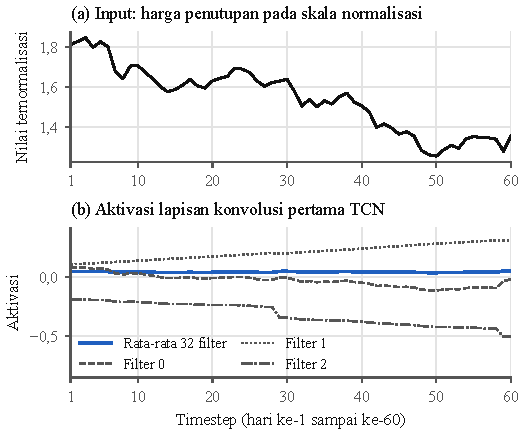
\includegraphics[width=\columnwidth]{fig5_aktivasi.pdf}
\caption{(a) Input harga dan (b) aktivasi lapisan konvolusi pertama TCN pada sampel test terakhir.}
\label{fig:aktivasi}
\end{figure}

\section{Keterbatasan Penelitian}
\label{sec:keterbatasan}
Hasil penelitian perlu dibaca dengan memperhatikan tujuh keterbatasan berikut.
\begin{enumerate}
\item \textbf{Target berupa harga mentah.} Sebanyak 56,5\% harga setelah batas fit scaler melebihi harga tertinggi data fit (67.566,83 USD). Model harus berekstrapolasi di luar rentang yang dipelajarinya.
\item \textbf{Satu pembagian waktu.} Evaluasi hanya memakai satu periode test, sehingga belum mewakili semua kondisi pasar.
\item \textbf{Tidak ada eksperimen tanpa fitur siklis.} Dampak fitur waktu terhadap akurasi belum dapat diukur.
\item \textbf{Tidak ada penyetelan hyperparameter.} Validation split tidak dipakai untuk early stopping atau pemilihan model.
\item \textbf{Run terbaik dipilih dari data test.} Plot dan analisis interpretabilitas memakai run tersebut, sehingga cenderung lebih optimistis daripada kinerja rata-rata.
\item \textbf{Interpretabilitas masih terbatas.} SHAP hanya memakai 3 sampel test, sedangkan pembacaan t-SNE bersifat kualitatif.
\item \textbf{Batas scaler dan batas window sedikit berbeda.} Scaler di-fit pada 3.277 observasi pertama, sedangkan target training terakhir berada pada observasi ke-3.288, sehingga 11 target training berada di luar data fit.
\end{enumerate}

\section{Kesimpulan dan Saran}

\subsection{Kesimpulan}
Kesimpulan dijawab mengikuti lima rumusan masalah.
\begin{enumerate}
\item \textbf{Perbandingan model:} TCN mencatat error rata-rata terendah (RMSE 3.180,83 USD), diikuti LSTM (4.908,63 USD) dan RNN (7.378,45 USD).
\item \textbf{Perbandingan dengan baseline:} tidak satu pun dari 15 run mengalahkan baseline persistence (RMSE 1.913,46 USD).
\item \textbf{Stabilitas antar-seed:} simpangan baku RMSE TCN adalah yang terkecil, tetapi LSTM mengungguli TCN pada seed 1234.
\item \textbf{Fitur berpengaruh menurut SHAP:} harga penutupan mendominasi prediksi TCN, walaupun hasil ini hanya berasal dari 3 sampel.
\item \textbf{Pemisahan tren pada representasi laten:} secara visual, tidak ada model yang memisahkan hari naik dan hari turun.
\end{enumerate}

\subsection{Saran}
\begin{enumerate}
\item Mengganti target menjadi return atau log-return agar model tidak bergantung pada level harga.
\item Menguji model dengan walk-forward validation pada beberapa periode pasar.
\item Melakukan eksperimen dengan dan tanpa fitur siklis untuk mengukur kontribusinya.
\item Memakai data validasi untuk early stopping, penyetelan hyperparameter, dan pemilihan model.
\item Memperluas analisis SHAP ke lebih banyak sampel dan menilai pemisahan tren secara kuantitatif.
\item Menambahkan fitur lain, seperti volume, data on-chain, sentimen pasar, atau fase halving.
\end{enumerate}

\IEEEtriggeratref{5}
\begin{thebibliography}{13}

\bibitem{nakamoto2008}
S. Nakamoto, ``Bitcoin: A peer-to-peer electronic cash system,'' 2008. [Online]. Tersedia: https://bitcoin.org/bitcoin.pdf

\bibitem{lim2021}
B. Lim dan S. Zohren, ``Time-series forecasting with deep learning: A survey,'' \textit{Philos. Trans. Roy. Soc. A}, vol. 379, no. 2194, Art. no. 20200209, 2021.

\bibitem{bai2018}
S. Bai, J. Z. Kolter, dan V. Koltun, ``An empirical evaluation of generic convolutional and recurrent networks for sequence modeling,'' arXiv:1803.01271, 2018.

\bibitem{hyndman2021}
R. J. Hyndman dan G. Athanasopoulos, \textit{Forecasting: Principles and Practice}, ed. ke-3. OTexts, 2021. [Online]. Tersedia: https://otexts.com/fpp3/

\bibitem{elman1990}
J. L. Elman, ``Finding structure in time,'' \textit{Cogn. Sci.}, vol. 14, no. 2, hlm. 179--211, 1990.

\bibitem{bengio1994}
Y. Bengio, P. Simard, dan P. Frasconi, ``Learning long-term dependencies with gradient descent is difficult,'' \textit{IEEE Trans. Neural Netw.}, vol. 5, no. 2, hlm. 157--166, 1994.

\bibitem{hochreiter1997}
S. Hochreiter dan J. Schmidhuber, ``Long short-term memory,'' \textit{Neural Comput.}, vol. 9, no. 8, hlm. 1735--1780, 1997.

\bibitem{gers2000}
F. A. Gers, J. Schmidhuber, dan F. Cummins, ``Learning to forget: Continual prediction with LSTM,'' \textit{Neural Comput.}, vol. 12, no. 10, hlm. 2451--2471, 2000.

\bibitem{fama1970}
E. F. Fama, ``Efficient capital markets: A review of theory and empirical work,'' \textit{J. Finance}, vol. 25, no. 2, hlm. 383--417, 1970.

\bibitem{hodson2022}
T. O. Hodson, ``Root-mean-square error (RMSE) or mean absolute error (MAE): When to use them or not,'' \textit{Geosci. Model Dev.}, vol. 15, no. 14, hlm. 5481--5487, 2022.

\bibitem{hyndman2006}
R. J. Hyndman dan A. B. Koehler, ``Another look at measures of forecast accuracy,'' \textit{Int. J. Forecasting}, vol. 22, no. 4, hlm. 679--688, 2006.

\bibitem{lundberg2017}
S. M. Lundberg dan S.-I. Lee, ``A unified approach to interpreting model predictions,'' dalam \textit{Proc. Adv. Neural Inf. Process. Syst.}, vol. 30, 2017, hlm. 4765--4774.

\bibitem{vandermaaten2008}
L. van der Maaten dan G. Hinton, ``Visualizing data using t-SNE,'' \textit{J. Mach. Learn. Res.}, vol. 9, no. 86, hlm. 2579--2605, 2008.

\end{thebibliography}

\end{document}
